\section{Overview of Mining GCMP in Parallel}
\label{sec:system_overview}
We adapt the MapReduce paradigm for designing
a parallel solution of mining GCMP. 
MapReduce was proposed by Dean et. cl.~\cite{dean2008mapreduce}
and has become a mature parallel platform for large-scaled data processing. 
Current open source MapReduce systems provide handy programming APIs with fault tolerances
in backends. Such systems include Hadoop, Shark and Spark to name a few.

In simple words, there are two types of computing nodes in MapReduce,
namely the \emph{mapper}s and the \emph{reducer}s. The execution of a MapReduce task consists of
three stages: First, input data
are partitioned and read by a \emph{map} function on each mapper. Then, mappers
emit key-value pairs which are \emph{shuffle}d over the network to reducers. Finally,
reducers process received data using a \emph{reduce} function then write the
outputs.
Since the \emph{shuffle} stage needs to transfer data over network, 
an important attention to pay during designing MapReduce an algorithm is 
to minimize the shuffle amounts and shuffle counts. 

Our GCMP mining framework consists of two MapReduce jobs which
are constituted of four MapReduce stages as illlustrated in Figure~\ref{fig:overview}.
The first MapReduce job corresponds to Figures~\ref{fig:overview}(a)-(b). The objective
of the first job is to cluster trajectories based on snapshots (i.e., computing $\forall t, o, C_t(o)$).
As illustrated in (a), input trajectories are read in by mappers 
and are sprinkled into $\langle t,o \rangle$ pairs. In (b), objects with the same timestamp
form a snapshot. Then, a user defined clustering method is applied on the objects
in each snapshot in reducers. Between step (a) and (b), a shuffle is necessary. The second
MapReduce job corresponds to Figures~\ref{fig:overview} (c)-(d). The objective 
of the second job is to mine the GCMP from the snapshots computed in the first job. We design
two approaches (to be described shortly)for mining GCMP in parallel. In overview, as shown in (c), snapshots
are first fed to mappers and different partition strategies may be selected to create
partitions among snapshots. In (d), the partitions are then send to reducers to mine GCMP.
The final computed results are then outputted to the end users. Although we need two MapReduce
jobs for a complete GCMP mining framework, we may pipeline the two jobs to exploit the data locality.
Specifically, the reducer output at step (b) can be directly reused as the input to mappers at step (c). Therefore
we do not need to transfer data from step (b) to step (c). Modern MapReduce platforms, especially Spark, have
already supported such a kind of pipeline.

\begin{figure} [t]
\center
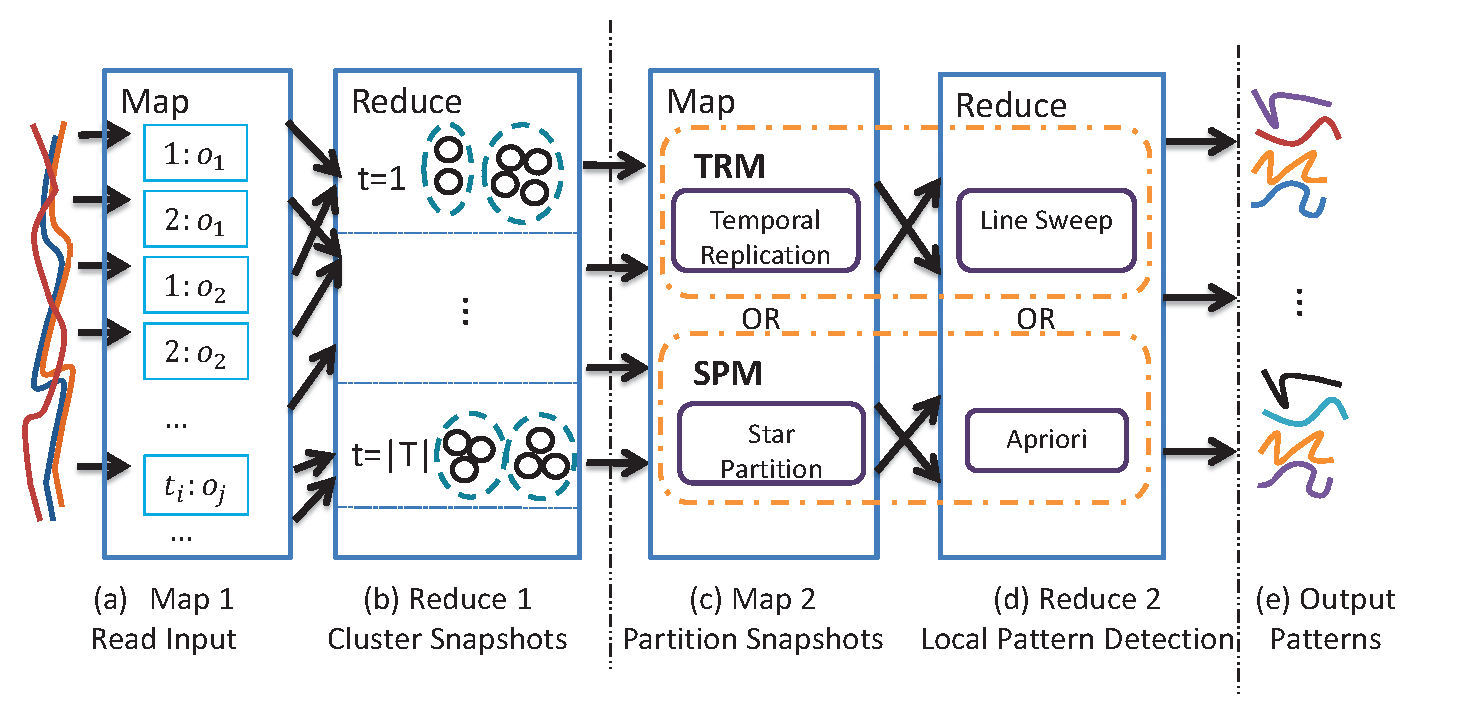
\includegraphics[width=0.5\textwidth]{system_layout.eps}
\caption{System flow of mining GCMP}
\label{fig:overview}
\end{figure}



The first MapReduce job to compute clusters in each snapshot
is easy to work in parallel. This is because a clustering method only needs
to access data within in a snapshot. 
In contrast, it is challenging
to design a partition-and-mining methods for the second job. This is because
valid patterns may spray across multiple snapshots, where inappropraite partition
may fail to discover some valid patterns.
Formally, a reasonable partition strategy 
needs to meet the following requirements: first, the resulted partitions need
to preserve enough information so that real patterns can be discovered in the reduce phase. 
Second, the resulted partitions need to ensure that
the patterns discovered in the reduce phase are real patterns so that
no further validation is required. We formalize the two 
properties as \emph{completeness} and \emph{soundness} as follows:

\begin{definition}[Completeness and Soundness]
Let a partition method $\mathbb{P}$ partitions original trajectories $Tr$ into multiple parts, $Par_1,...,Par_m$. $\mathbb{P}$ is complete if for every pattern $P$ that is valid in $Tr$, $\exists Par_i$ such that $P$ is valid in $Par_i$. $\mathbb{P}$ is sound if for all patterns $P$ that is valid in any $Par_i$, it is also valid in $TR$.
\end{definition}
The completeness ensures that no true patterns are missed out. The soundness ensures that no false patterns are reported. 
If a partition method is both sound and complete, we are then able to design a MapReduce algorithm to facilitate the second job
of our framework.

Apparently, replicating the entire trajectories to each 
partition meets the \emph{soundness} and \emph{completeness}. However, 
it burdens the network shuffle and limits the parallelism. 
Our objective is thus to design a complete and sound partition method that minimize the network shuffles.
In the following sections, we first present a naive \emph{temporal-based} partition-and-mining method called \emph{Temporal Replication and Mining}(TRM) towards a parallel solution of GCMP mining. Then,
we further present a novel \emph{object-based} partition-and-mining method
called \emph{Star Partition and Mining} (SPM) which resolves
the deficiency of TRM method.

%Depends on the pattern mining strategy, the size of shuffle and replication may differ. We show that if the pattern mining strategy is not selected carefully, the second stage will suffer from large data replication and shuffling.


%
%In particular, we need
%the number of partitions to be reasonably large in order to achieve
%good parallelism in stage (d). Meanwhile, we need to ensure a partition 
%of snapshots containing enough information so that patterns discovered 
%in stage (d) are complete.  Furthermore, we have to ensure that the
%patterns that discovered in stage (d) are real patterns.

%However, there are two conflicting requirements that restrain us from 
%designing a simple and effective solution. 
%On one hand, we need to partition snapshots in stage (c) as many as possible 
%so that good parallelism could be achieved in stage (d). 
%On the other hand, in stage (d), 
%we require each partition containing enough information in order to discover
%proper GCMP patterns. This prevents us from arbitrarily partition snapshots in
%stage (d). To design a working algorithm, find the minimum size of partition is
%crucial. In the following section, we first design a naive approach that
%partitions snapshots by allowing overlapping among partitions. Such a partition strategy
%although has overhead in shuffling, it corrects find GCMPs in parallel in stage (d).
%In order to discover all patterns, we require a partitioning method to be \emph{complete} and \emph{Sound}. 

%\section{Temporal Replication and Mining}
%
%
%%It is notable that some patterns 
%%may be very long in duration (e.g., when discovering \emph{swarm}) or some patterns 
%%may contain a large set of objects (e.g., when discover \emph{group} patterns with small $L$).
%%Therefore, we require the size of partition to be large enough. Reaching the
%%balance between the two requirement is crucial. In the following sections, we will
%%describe a naive partition scheme which meets the two requirements.
%
%%Our parallel solution incurs two rounds of shuffles. The first round of shuffle happens in step (a). This
%%is because that the trajectories stored in HDFS needs to be regrouped to form snapshots. 
%%The second round of shuffle occurs in step(d). This is because that 
%% the clusters need to be regrouped so that subsequent pattern detection can be performed.
%% Despite the simpleness of our parallel solution, it is actually nontrivial to work out a scalable solution.
%% The major challenge lies in the step (d) and (e). 
%
%
%%\section{Preliminary on Apache Spark}
%%\label{sec:system_overview}
%%Apache Spark is an open sourced modern parallel processing platform
%%based on Resilient-Distributed-Dataset (RDD). Each RDD is able to take an action (including Map, Reduce, GroupByKey etc.) and then transforms to a new RDD. Algorithms in Spark is implemented by supplying various actions to an input RDD. Each RDD in Spark has a pre-defined and fixed number of partitions, where each partition forms a task assigned to an executor.
%%
%%Compared to MapReduce, Spark 
%%utilizes distributed memory to cache the programming data modeled as RDDs, which brings computational benefits~\cite{shi2015clash}. In order to fully utilize the memory, Spark creates one thread for each task and then multiple tasks belonging to the same JVM share the available memory.
%Due to threading, there is a paradigm shift from MapReduce to Spark. In MapReduce, the cost of starting a task is expensive, as each task in MapReduce requires a dedicated JVM process. While in Spark, the cost of starting a task is negligible since each task is done by a thread.  Therefore in Spark, we may create many more parallel tasks than in MapReduce before reaching to the system limitation.


%\section{Mining Generalized Co-moving Pattern}
%\label{sec:solution}
%There are two stages in mining GCMP. The first stage is to cluster objects in each snapshots. Then the seconds stage is to mine patterns from clusters in parallel. The overview of the parallel approach is 
%shown in Figure~\ref{fig:overview}. As shown, trajectory data is initially stored in HDFS. The first stage is to 
%read trajectories and cluster objects in the same snapshots. Since the objects at each snapshots are independent, this stage can be easily performed in parallel. The first stage involves network IO. Afterwards, the clusters in each snapshots are shuffled and replicated to make various partitions.



